\documentclass[11pt,a4paper]{article}
\usepackage[T1]{fontenc}
\usepackage{lmodern}
\usepackage[margin=2.3cm]{geometry}
\usepackage{microtype}
\usepackage{amsmath}
\usepackage{graphicx}
\usepackage{xcolor}
\usepackage{enumitem}
\usepackage[colorlinks=true,urlcolor=blue!50!black,linkcolor=black]{hyperref}
\graphicspath{{../figures/}}
\setlength{\parindent}{0pt}
\setlength{\parskip}{0.7em}
\pagestyle{plain}

\begin{document}

\begin{center}
{\LARGE\bfseries Hunting the Faintest Galaxies:\\[0.3em] New Milky Way Satellites in Euclid DR1}
\end{center}
\vspace{0.5em}

The Milky Way is surrounded by a swarm of small companion galaxies. The faintest of them, the ultra-faint dwarf galaxies, are among the most extreme objects in the Universe: some shine with the light of only a few hundred Suns, yet their stars move as if held by a mass hundreds to thousands of times larger. They are dominated by dark matter, and their stars are old and poor in heavy elements, relics of the first galaxies to form. They are far too faint to see as a glow on the sky. Instead, they reveal themselves as a slight excess of individual stars, of the right colour and brightness, against the much more numerous stars of our own Galaxy and the faint background galaxies behind them (Simon 2019). The aim of this project is to discover new ultra-faint dwarfs, and as a second goal new stellar streams, in the first large data release of the Euclid space telescope, which arrives during the academic year.

Ultra-faint dwarfs matter for four reasons. The first is the \emph{missing satellites problem}. Cosmological simulations of cold dark matter predict that a galaxy like the Milky Way should be surrounded by hundreds to thousands of small dark-matter clumps, or subhaloes, yet in 1999 only about a dozen satellites were known (Klypin et al.\ 1999; Moore et al.\ 1999). Two things close the gap. Only some subhaloes can host stars, because in the smallest ones the ultraviolet radiation that reionised the Universe heated the gas before it could cool and form stars. And most faint satellites have simply not been found yet. Once the known ultra-faint dwarfs are corrected for the parts of the sky and the depths that surveys have missed, their numbers agree with cold dark matter (Kim, Peter \& Hargis 2018). The same counts set limits on alternatives: if dark matter were ``warm'' (its particles moving fast in the early Universe) or if its particles interacted with each other, the smallest subhaloes would never form, and the faintest satellites would be missing. Comparisons with simulations of Milky Way-like haloes already turn the known satellites into some of the strongest limits on the properties of dark matter (Bullock \& Boylan-Kolchin 2017; Jethwa, Erkal \& Belokurov 2018; Nadler et al.\ 2021). Every new ultra-faint dwarf tightens these limits.

The other three reasons concern galaxy formation itself. Ultra-faint dwarfs are the oldest galaxies we can study star by star. In those with deep Hubble photometry, about 80 per cent of the stars formed more than 12.8 billion years ago, before the end of reionisation, and star formation then stopped (Brown et al.\ 2014). Some may be surviving fossils of the first galaxies, which formed before reionisation (Bovill \& Ricotti 2009). They also formed stars under extreme physical conditions: in the smallest dark-matter haloes able to form stars at all, from gas almost free of heavy elements, and with so few stars that a single supernova or neutron-star merger could change the composition of the whole galaxy. As a result their chemistry can be unlike anything else in the Milky Way. In the ultra-faint dwarf Reticulum~II, seven of the nine brightest stars carry 100 to 1000 times more rapid-neutron-capture ($r$-process) elements, such as europium, than stars in other ultra-faint dwarfs. A single rare event, most likely a neutron-star merger, enriched the entire galaxy (Ji et al.\ 2016). Such stars record the elements made by the first generations of stars (Frebel \& Norris 2015). Each new ultra-faint dwarf adds a new, independent experiment in early galaxy formation.

The dark-matter limits rest on a correction. Only part of the sky has been searched deeply enough, and a search finds a nearby, compact dwarf far more easily than a distant, diffuse one. To get from the satellites we have found to the total number that exists, we need to know the efficiency of each search, its \emph{selection function}. The standard way to measure it is to insert artificial galaxies into the real data and count how many the search recovers (Drlica-Wagner et al.\ 2020). At present, our poor knowledge of where faint satellites lie, and how far out they can be found, contributes more uncertainty to the dark-matter constraints than the detections themselves.

The search technique was developed on large digital sky surveys such as SDSS and DES (Koposov et al.\ 2008, 2015; Torrealba et al.\ 2016a, 2016b; Cerny et al.\ 2021, 2023). It uses the colour--magnitude diagram, the observer's version of the Hertzsprung--Russell diagram. All stars in a dwarf galaxy formed at about the same time from gas of about the same composition, so they lie along a single curve, an \emph{isochrone}, in this diagram. For a trial distance $d$ the isochrone shifts in apparent magnitude by the distance modulus $m - M = 5\log_{10}(d/10\,\mathrm{pc})$. Selecting stars close to the shifted curve and mapping their positions on the sky boosts the contrast of any dwarf at that distance. Smoothing the map on two angular scales and subtracting one from the other removes the slowly varying Galactic foreground and leaves compact peaks. Each peak is then checked: does its colour--magnitude diagram follow an isochrone, does it persist when the selection changes, do the brighter stars share a common motion in Gaia, and is it an artefact or a group of background galaxies? Figure~\ref{fig:bootes} shows a recent discovery made in exactly this way.

\begin{figure}[t]
\centering
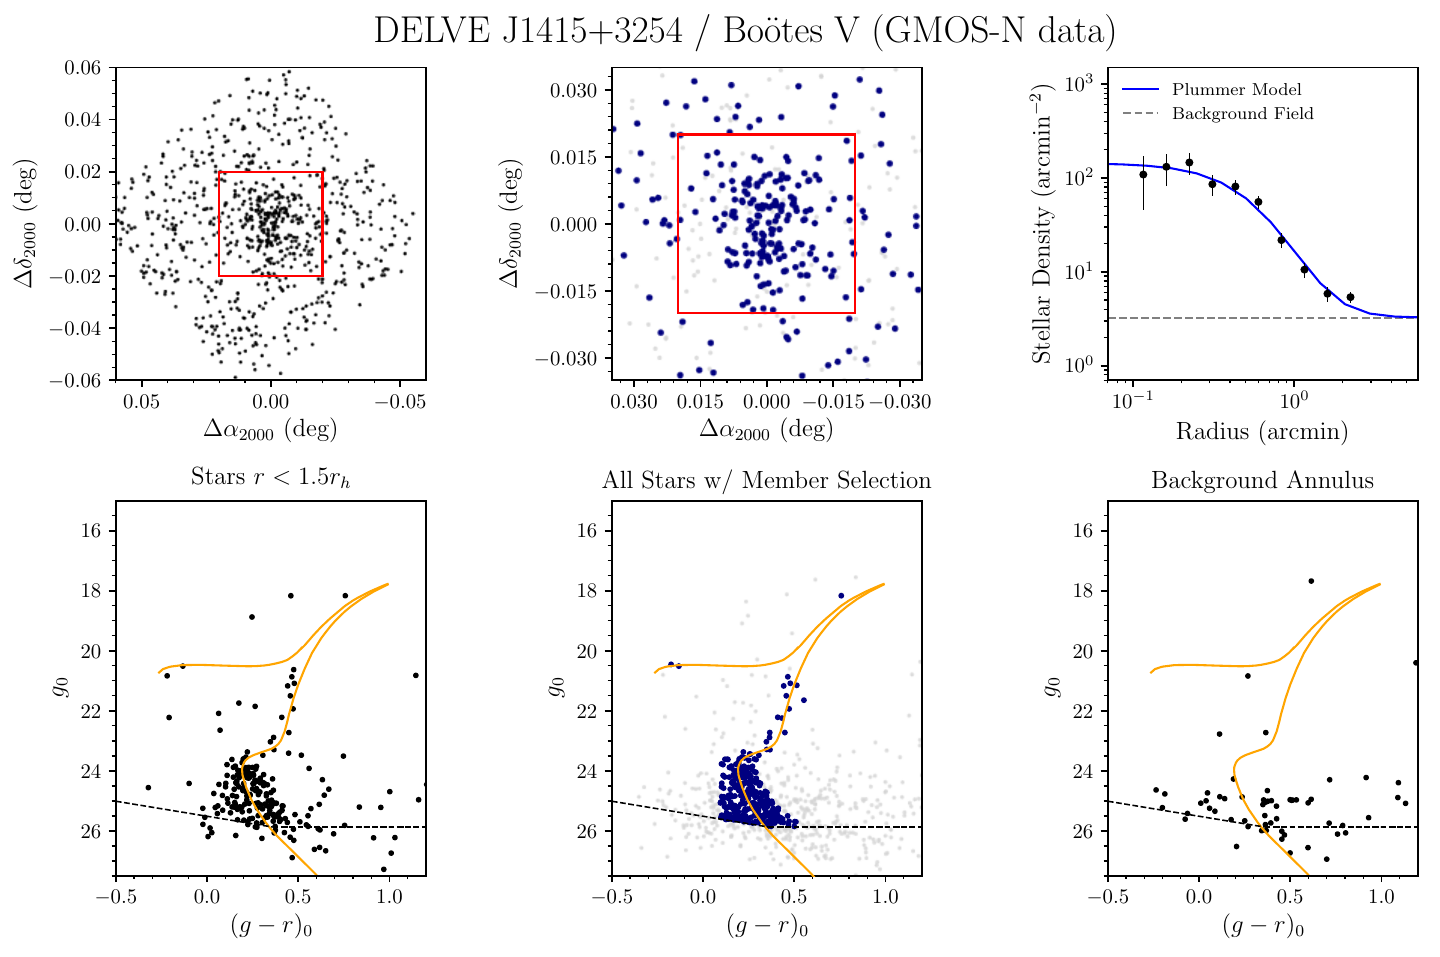
\includegraphics[width=0.9\textwidth]{01_cerny2023_bootesV_discovery.png}
\caption{\small Discovery of the ultra-faint dwarf Bo\"otes~V in the DELVE survey. Top: the clump of isochrone-selected stars on the sky and its density profile against the background. Bottom: colour--magnitude diagrams of the central region, of the likely members, and of a comparison field, with an old, metal-poor isochrone (orange). The Euclid search uses the same steps, pushed to fainter and more distant systems. From Cerny et al.\ (2023).}
\label{fig:bootes}
\end{figure}

The ESA Euclid space telescope will push this experiment further than any survey so far. Euclid is mapping about a third of the sky with sharp optical images (its VIS camera) and near-infrared photometry (its NISP instrument), reaching stars far fainter than Gaia can see (Scaramella et al.\ 2022). The hardest problem in a search for ultra-faint dwarfs is that, at faint magnitudes, distant galaxies look like stars from the ground. Euclid's space-based resolution separates the two much better, so the student can count fainter stars and therefore detect smaller, fainter and more distant dwarfs. The first major Euclid data release, DR1, begins in November 2026 and is completed in mid-2027. The student will build and test the search on public data available now, including the Euclid Quick Release Q1 (Aussel et al.\ 2026), and then turn it on DR1 as it appears. No one will yet have searched these data for faint satellites. This project is designed to be that first search, and any convincing system it finds will be a new member of the Milky Way's family of companions.

The student will write a transparent search pipeline, measure its sensitivity by injecting and recovering artificial dwarf galaxies, rank every credible candidate, and estimate the distance, size, shape, and luminosity of the strongest ones. The measured sensitivity is what links the discoveries back to theory: it allows the results to be compared directly with the satellite populations predicted by dark-matter simulations. Some candidates may turn out to be faint star clusters instead of galaxies; telling the two apart, by whether they contain dark matter, will need follow-up spectroscopy, and the project will produce a priority list for it.

The second discovery target is stellar streams. When the Milky Way's tides tear apart a dwarf galaxy or a star cluster, its stars spread along the orbit into a long, thin, faint band across the sky. The same isochrone-selected star maps that reveal compact dwarfs also show these elongated features, and wide-field surveys have found many streams this way (Shipp et al.\ 2018). Because a stream's stars follow nearly the same orbit, the stream traces the gravitational field it moves through, and it is one of the best tools for weighing the Milky Way. Streams answer three questions about the Galaxy's dark matter.
\begin{itemize}[leftmargin=1.2em,itemsep=0.2em,parsep=0pt,topsep=0.2em]
\item \emph{How much mass is there, and where?} Fitting the orbit of the GD-1 stream measured the Galaxy's circular velocity and the flattening of its potential about 15\,kpc from the centre (Koposov, Rix \& Hogg 2010).
\item \emph{What is the three-dimensional shape of the dark-matter halo?} Each stream samples the force field along its own path, so streams at different distances and orientations map the halo's shape. Results so far disagree: models of the Sagittarius stream required a flattened, triaxial halo (Law \& Majewski 2010), while the Pal~5 and GD-1 streams favour a nearly spherical halo within 20\,kpc (Bovy et al.\ 2016).
\item \emph{How does the dark matter change with time?} The Large Magellanic Cloud, with a total mass above $10^{11}\,M_\odot$, is falling into the Milky Way. It has bent the Orphan stream (Erkal et al.\ 2019) and pulls the Milky Way towards it, so the Sagittarius stream cannot be modelled in a static Galaxy (Vasiliev, Belokurov \& Erkal 2021). Streams therefore record a potential that is still changing.
\end{itemize}
Thin streams also test dark matter on the smallest scales. Each time a small dark-matter subhalo flies past, it opens a gap in the stream, so the number and size of gaps measure how many dark subhaloes, too small to host any stars, orbit the Galaxy (Erkal et al.\ 2016). Every new stream adds a new probe at a new position in the halo. Euclid's depth should reveal streams too faint and too distant for earlier surveys, including in the outer halo, where the pull of the Large Magellanic Cloud matters most. Once the dwarf-galaxy search is complete, the student will reuse the validated star maps to search for them.

The project suits a student who enjoys programming in Python and working with large data sets. Experience with colour--magnitude diagrams or astronomical catalogues helps but is not required.

\vspace{0.5em}
{\small\raggedright
\textbf{Further reading}
\begin{itemize}[leftmargin=1.2em,itemsep=0.1em,parsep=0pt,topsep=0.3em]
\item Simon, J.\,D. (2019), \emph{The Faintest Dwarf Galaxies}, ARA\&A, 57, 375. \href{https://doi.org/10.1146/annurev-astro-091918-104453}{doi:10.1146/annurev-astro-091918-104453}
\item Bullock, J.\,S. \& Boylan-Kolchin, M. (2017), \emph{Small-Scale Challenges to the $\Lambda$CDM Paradigm}, ARA\&A, 55, 343. \href{https://doi.org/10.1146/annurev-astro-091916-055313}{doi:10.1146/annurev-astro-091916-055313}
\item Klypin, A. et al.\ (1999), \emph{Where Are the Missing Galactic Satellites?}, ApJ, 522, 82. \href{https://doi.org/10.1086/307643}{doi:10.1086/307643}
\item Moore, B. et al.\ (1999), \emph{Dark Matter Substructure within Galactic Halos}, ApJ, 524, L19. \href{https://doi.org/10.1086/312287}{doi:10.1086/312287}
\item Kim, S.\,Y., Peter, A.\,H.\,G. \& Hargis, J.\,R. (2018), \emph{Missing Satellites Problem: Completeness Corrections to the Number of Satellite Galaxies in the Milky Way are Consistent with Cold Dark Matter Predictions}, Phys.\ Rev.\ Lett., 121, 211302. \href{https://doi.org/10.1103/PhysRevLett.121.211302}{doi:10.1103/PhysRevLett.121.211302}
\item Brown, T.\,M. et al.\ (2014), \emph{The Quenching of the Ultra-faint Dwarf Galaxies in the Reionization Era}, ApJ, 796, 91. \href{https://doi.org/10.1088/0004-637X/796/2/91}{doi:10.1088/0004-637X/796/2/91}
\item Bovill, M.\,S. \& Ricotti, M. (2009), \emph{Pre-Reionization Fossils, Ultra-Faint Dwarfs, and the Missing Galactic Satellite Problem}, ApJ, 693, 1859. \href{https://doi.org/10.1088/0004-637X/693/2/1859}{doi:10.1088/0004-637X/693/2/1859}
\item Ji, A.\,P., Frebel, A., Chiti, A. \& Simon, J.\,D. (2016), \emph{R-process enrichment from a single event in an ancient dwarf galaxy}, Nature, 531, 610. \href{https://doi.org/10.1038/nature17425}{doi:10.1038/nature17425}
\item Frebel, A. \& Norris, J.\,E. (2015), \emph{Near-Field Cosmology with Extremely Metal-Poor Stars}, ARA\&A, 53, 631. \href{https://doi.org/10.1146/annurev-astro-082214-122423}{doi:10.1146/annurev-astro-082214-122423}
\item Jethwa, P., Erkal, D. \& Belokurov, V. (2018), \emph{The upper bound on the lowest mass halo}, MNRAS, 473, 2060. \href{https://doi.org/10.1093/mnras/stx2330}{doi:10.1093/mnras/stx2330}
\item Nadler, E.\,O. et al.\ (2021), \emph{Constraints on Dark Matter Properties from Observations of Milky Way Satellite Galaxies}, Phys.\ Rev.\ Lett., 126, 091101. \href{https://doi.org/10.1103/PhysRevLett.126.091101}{doi:10.1103/PhysRevLett.126.091101}
\item Koposov, S. et al.\ (2008), \emph{The Luminosity Function of the Milky Way Satellites}, ApJ, 686, 279. \href{https://doi.org/10.1086/589911}{doi:10.1086/589911}
\item Koposov, S.\,E. et al.\ (2015), \emph{Beasts of the Southern Wild: Discovery of nine ultra-faint satellites in the vicinity of the Magellanic Clouds}, ApJ, 805, 130. \href{https://doi.org/10.1088/0004-637X/805/2/130}{doi:10.1088/0004-637X/805/2/130}
\item Torrealba, G. et al.\ (2016a), \emph{The Feeble Giant: Discovery of a large and diffuse Milky Way dwarf galaxy in the constellation of Crater}, MNRAS, 459, 2370. \href{https://doi.org/10.1093/mnras/stw733}{doi:10.1093/mnras/stw733}
\item Torrealba, G. et al.\ (2016b), \emph{At the survey limits: discovery of the Aquarius 2 dwarf galaxy in the VST ATLAS and the SDSS data}, MNRAS, 463, 712. \href{https://doi.org/10.1093/mnras/stw2051}{doi:10.1093/mnras/stw2051}
\item Drlica-Wagner, A. et al.\ (2020), \emph{Milky Way Satellite Census.\ I.\ The Observational Selection Function for Milky Way Satellites in DES Y3 and Pan-STARRS DR1}, ApJ, 893, 47. \href{https://doi.org/10.3847/1538-4357/ab7eb9}{doi:10.3847/1538-4357/ab7eb9}
\item Cerny, W. et al.\ (2021), \emph{Eridanus IV: An Ultra-Faint Dwarf Galaxy Candidate Discovered in the DECam Local Volume Exploration Survey}, ApJL, 920, L44. \href{https://doi.org/10.3847/2041-8213/ac2d9a}{doi:10.3847/2041-8213/ac2d9a}
\item Cerny, W. et al.\ (2023), \emph{Six More Ultra-Faint Milky Way Companions Discovered in the DECam Local Volume Exploration Survey}, ApJ, 953, 1. \href{https://doi.org/10.3847/1538-4357/acdd78}{doi:10.3847/1538-4357/acdd78}
\item Shipp, N. et al.\ (2018), \emph{Stellar Streams Discovered in the Dark Energy Survey}, ApJ, 862, 114. \href{https://doi.org/10.3847/1538-4357/aacdab}{doi:10.3847/1538-4357/aacdab}
\item Koposov, S.\,E., Rix, H.-W. \& Hogg, D.\,W. (2010), \emph{Constraining the Milky Way Potential with a Six-Dimensional Phase-Space Map of the GD-1 Stellar Stream}, ApJ, 712, 260. \href{https://doi.org/10.1088/0004-637X/712/1/260}{doi:10.1088/0004-637X/712/1/260}
\item Law, D.\,R. \& Majewski, S.\,R. (2010), \emph{The Sagittarius Dwarf Galaxy: A Model for Evolution in a Triaxial Milky Way Halo}, ApJ, 714, 229. \href{https://doi.org/10.1088/0004-637X/714/1/229}{doi:10.1088/0004-637X/714/1/229}
\item Bovy, J., Bahmanyar, A., Fritz, T.\,K. \& Kallivayalil, N. (2016), \emph{The Shape of the Inner Milky Way Halo from Observations of the Pal 5 and GD-1 Stellar Streams}, ApJ, 833, 31. \href{https://doi.org/10.3847/1538-4357/833/1/31}{doi:10.3847/1538-4357/833/1/31}
\item Erkal, D. et al.\ (2019), \emph{The total mass of the Large Magellanic Cloud from its perturbation on the Orphan stream}, MNRAS, 487, 2685. \href{https://doi.org/10.1093/mnras/stz1371}{doi:10.1093/mnras/stz1371}
\item Vasiliev, E., Belokurov, V. \& Erkal, D. (2021), \emph{Tango for three: Sagittarius, LMC, and the Milky Way}, MNRAS, 501, 2279. \href{https://doi.org/10.1093/mnras/staa3673}{doi:10.1093/mnras/staa3673}
\item Erkal, D., Belokurov, V., Bovy, J. \& Sanders, J.\,L. (2016), \emph{The number and size of subhalo-induced gaps in stellar streams}, MNRAS, 463, 102. \href{https://doi.org/10.1093/mnras/stw1957}{doi:10.1093/mnras/stw1957}
\item Scaramella, R. et al.\ (2022), \emph{Euclid preparation.\ I.\ The Euclid Wide Survey}, A\&A, 662, A112. \href{https://doi.org/10.1051/0004-6361/202141938}{doi:10.1051/0004-6361/202141938}
\item Aussel, H. et al.\ (2026), \emph{Euclid Quick Data Release (Q1).\ I.\ Data release overview}, A\&A, 711, A1. \href{https://doi.org/10.1051/0004-6361/202554610}{doi:10.1051/0004-6361/202554610}
\item ESA, \emph{Euclid mission timeline and data releases}. \url{https://www.cosmos.esa.int/web/euclid/timeline}
\end{itemize}
}

\end{document}
